\subsection{Definition}
We consider the same test example definition as for isothermal gas flow in sec. \ref{bmt:Isothermal_compressible_flow}. Now we use pressure and temperature dependent material properties described in section \ref{bmt:G-material_functions}. The model parameters are summarized in Tab. \ref{tab:air_heat_1d}.
\begin{table}[h]
\caption{\label{tab:air_heat_1d}Model parameters}
\begin{center}
\begin{tabular}{llrr}
\toprule
Symbol & Parameter & Value & Unit \\
\midrule
$L$ & Model length & $100$ & $\mathrm{m}$\\
$n$ & Porosity & $0.35$  & $-$ \\
$\rho,\rho^s$ & Densities & (\ref{eqn:ideal_gas_law}), $2650$ & $\mathrm{kg~m^{-3}}$ \\
$\k$ & Permeability & $2.7\times 10^{-11}$ & $\mathrm{m^2}$\\
$\mu$ & Dynamic gas viscosity & (\ref{eqn:reichenberg_viscosity}) & $\mathrm{Pa~s}$\\
$p_0$ & Initial condition & $101325$ & $\mathrm{Pa}$\\
$T_0$ & Initial condition & $288$ & $\mathrm{K}$\\
$p_2$ & Boundary condition & $101325$ & $\mathrm{Pa}$\\
$T_1$ & Boundary condition & $343$ & $\mathrm{K}$\\
$Q_{\rho}$ & Injection rates & $1-10$ & $\mathrm{kg~s^{-1}}$\\
$\alpha_L, \alpha_T$ & Heat dispersion length & $1, 0.1$ & $\mathrm{m}$\\
$\lambda^g, \lambda^s$ & Heat conductivities & (\ref{eqn:thermal_conductivity}), $2.5$ & $\mathrm {W~m^{-1} K^{-1}}$\\
$c_p^g, c_p^s$ & Heat capacities & (\ref{eqn:heat_capacity}), $2300$ & $\mathrm {J kg^{-1} K^{-1}}$\\
\bottomrule
\end{tabular}
\end{center}
\end{table}
\subsection{Solution}
The numerical model consists of $100$ line elements connected by $101$ nodes along the x-axis. The distances of the nodes $\Delta x$ is one meter. At $x=0\mathrm {m}$, we injecting air with rates of $1~\mathrm {kg~s^{-1}}$ and $10~\mathrm {kg~s^{-1}}$, which temperature is $343~\mathrm K$. And at $x=L$, pressure boundary value is $1.01325 \times 10^5 \mathrm {Pa}$ and $\nabla T=0$.

\begin{figure}[htb!]
\includegraphics[scale=0.3]{PART_II/G/press_ply.eps}
\includegraphics[scale=0.3]{PART_II/G/velo_ply.eps}
\caption{Hydraulic profiles evolution: Air pressure (top), Air velocity (bottom).}
\label{fig:air_flow}
\end{figure}

\begin{figure}[htb!]
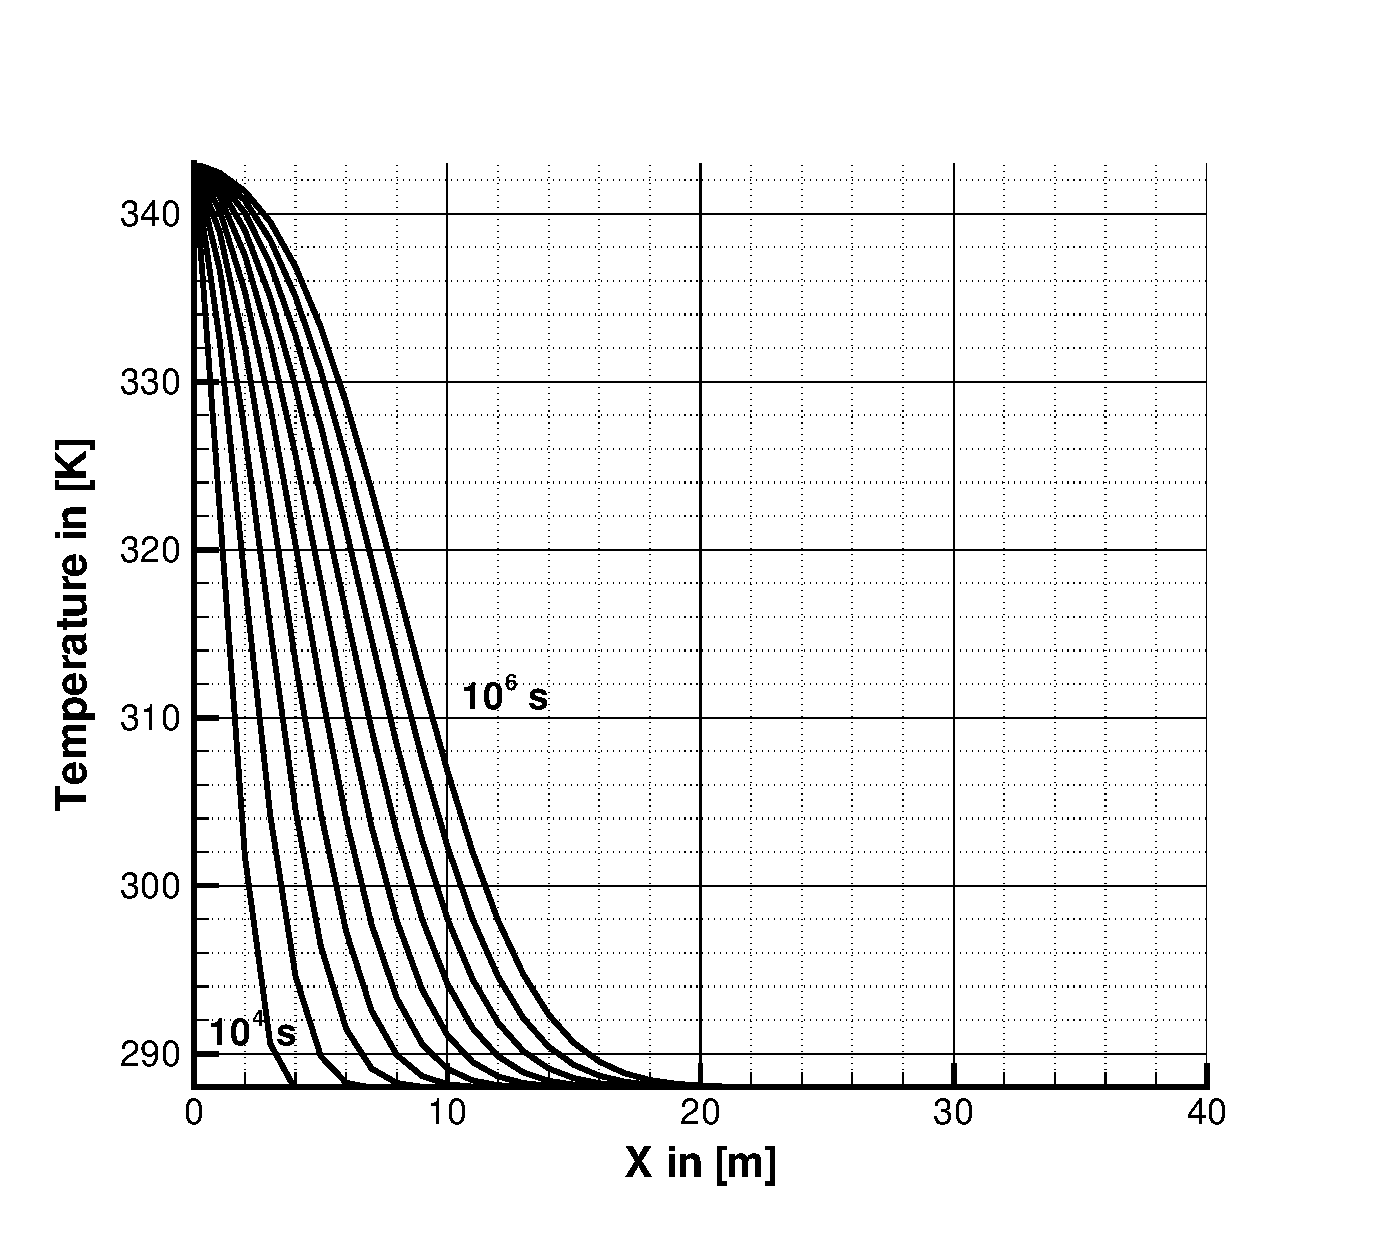
\includegraphics[scale=0.3]{PART_II/G/t_1.eps}
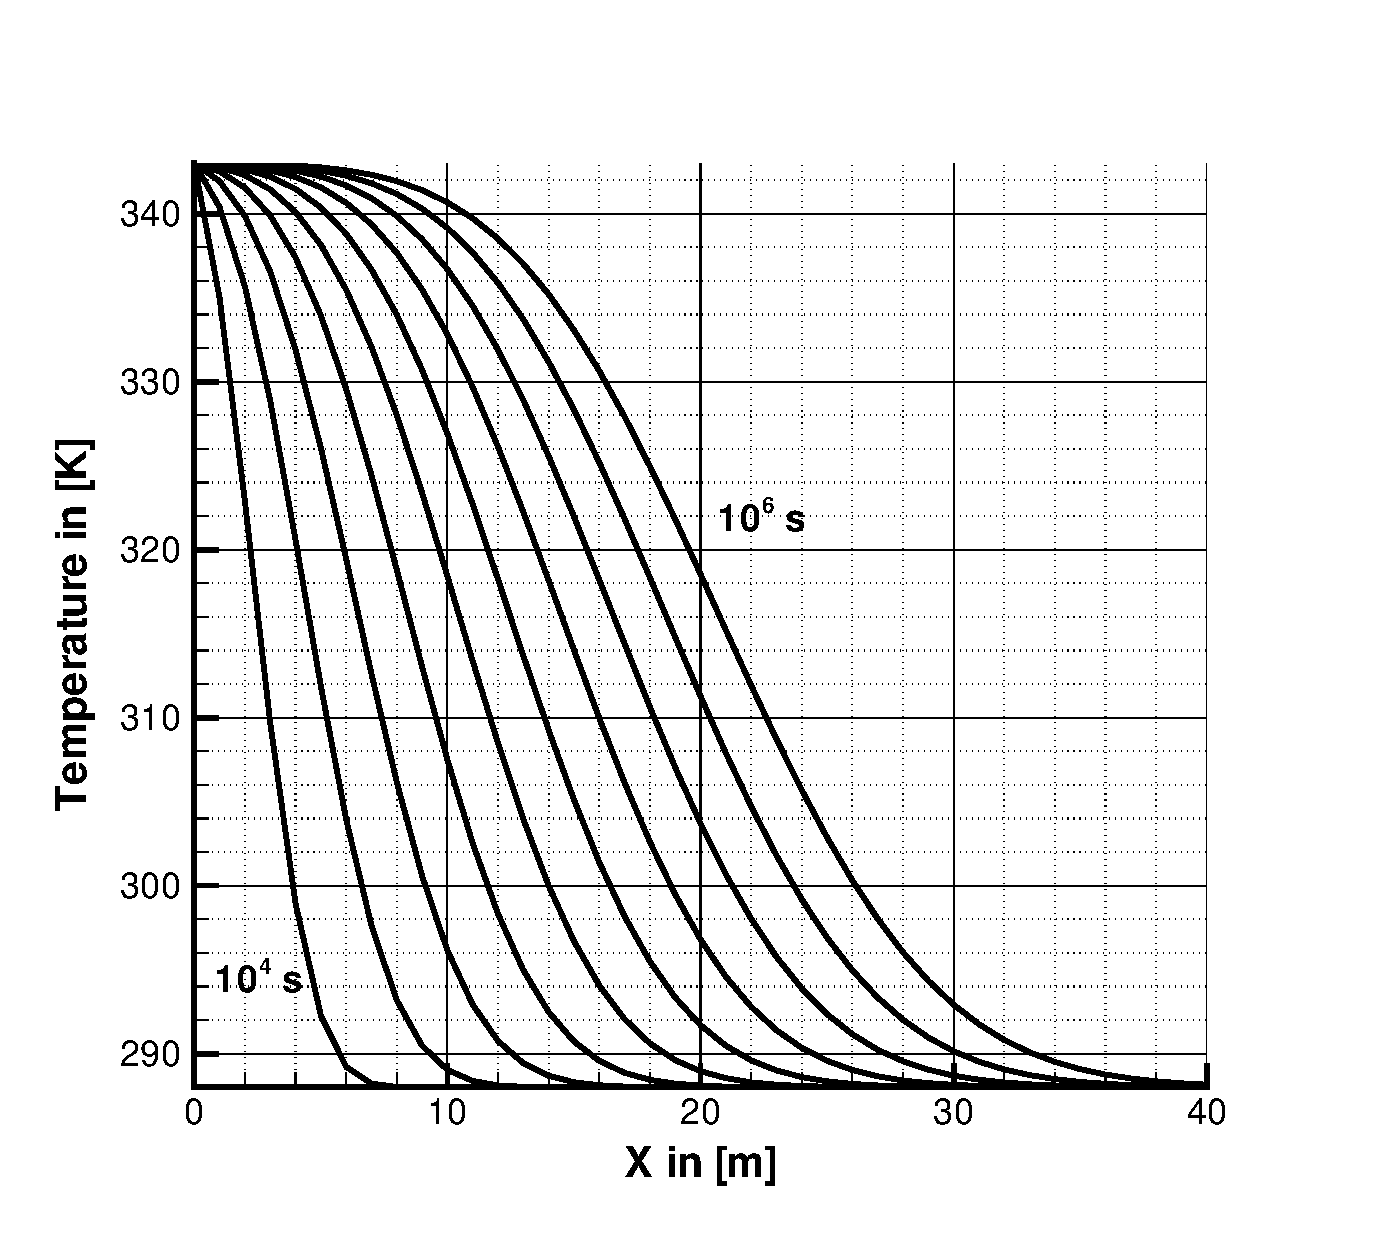
\includegraphics[scale=0.3]{PART_II/G/t_10.eps}
\caption{Air temperature profiles evolution. $1 \mathrm {kg~s^{-1}}$ air injection rate (top), $10 \mathrm {kg~s^{-1}}$ air injection rate (bottom).}
\label{fig:air_heat_1d_heat}
\end{figure}

\begin{figure}[htb!]
\begin{center}
\footnotesize
\includegraphics[width=0.5\columnwidth]{PART_II/G/non_isothermal_flow.eps}  % Filename.eps
\caption{Temporal evolution of air pressure profiles for non-isothermal gas flow.}
\label{fig:visco8}
\end{center}
\end{figure}

\subsection{Results}
Fig. \ref{fig:air_flow} show the air pressure (left) and velocity distributions (right) along the soil column. Simulations were run with constant viscosities and those corresponding to the Reichenberg model (section \ref{sec:Reichenberg_viscosity_model}) which takes pressure and temperature changes into account.


The corresponding temperature profiles for different air injection rates are depicted in Fig. \ref{fig:air_heat_1d_heat}. The different shapes of the thermal profile curves indicate the transition between diffusion (left) and advection dominated regimes (right).


Fig. \ref{fig:visco8} shows the temporal evolution of air pressure profile for non-isothermal air flow. In order to see the non-isothermal effects we plotted the analytical steady state solution for isothermal flow along with present numerical solution for non-isothermal flow. As a consequence of the viscosity increase resulting from the Reichenberg model the steady state pressure is larger for non-isothermal conditions.
